\section{度量张量}
\label{sec:metric_tensor}

在 \ref{sec:earth_system} 章中，我们认为地球系统是流形上的随机动力学过程。
为了更加深入地分析地球系统的几何结构，我们需要在流形 $\manifold$ 上定义距离、角度、体积、曲率等几何概念。
我们希望取得一个良好的定义，使得这些几何概念能够尽量充分地反映动力学过程的信息。

定义\textbf{度量张量 (Metric Tensor)} $\metric$。

\begin{definition}[度量张量]
\label{def:metric_tensor}
    度量张量 $g$ 是定义在流形切丛上的一个光滑、对称、正定的 $(0, 2)$ 型张量场。在局部坐标 $\bm{u} = (u^1, \ldots, u^k)$ 下，它表示为对称正定矩阵 $[\metric_{ij}(\bm{u})]$。
    两个无穷接近的点之间的距离平方为:
    \begin{equation}
    \label{eq:metric_tensor_def}
        ds^2 = \sum_{i,j=1}^k g_{ij}(\bm{u})\,du^i\,du^j = d\bm{u}^\top \metric(\bm{u}) d\bm{u}
    \end{equation}
\end{definition}

基于度量张量 $\metric$，我们定义\textbf{测地距离 (Geodesic Distance)} $d_\metric$。

\begin{definition}[测地距离]
\label{def:geodesic_distance}
    给定度量张量 $\metric$，流形 $\manifold$ 上两点 $p, q$ 之间的测地距离 $d_\metric(p, q)$ 定义为:
    \begin{equation}
    \label{eq:geodesic_distance}
        d_\metric(p, q) = \inf_{\gamma: p \to q} \int_0^1 \sqrt{\sum_{i,j=1}^k \metric_{ij}(\gamma(t)) \dot{\gamma}^i(t) \dot{\gamma}^j(t)}\, dt
    \end{equation}

    其中 $\gamma: [0,1] \to \manifold$ 是连接 $p = \gamma(0)$ 和 $q = \gamma(1)$ 的光滑曲线，$\dot{\gamma}(t) = \frac{d\gamma}{dt}$ 是切向量。
    测地距离是所有连接 $p$ 和 $q$ 的曲线中最短的弧长。
\end{definition}

我们定义\textbf{曲率 (Curvature)} 来刻画流形的弯曲程度 \cite{lee2018introduction}。

\begin{definition}[Riemann曲率张量]
\label{def:riemann_curvature_tensor}
    \begin{equation}
    \label{eq:riemann_curvature_tensor}
        R_{ijkl} = \frac{\partial \Gamma_{il}^m}{\partial x^k} - \frac{\partial \Gamma_{ik}^m}{\partial x^l} + \Gamma_{il}^n\Gamma_{nk}^m - \Gamma_{ik}^n\Gamma_{nl}^m
    \end{equation}

    其中 $\Gamma_{jk}^i = \frac{1}{2}g^{im}(\frac{\partial g_{mj}}{\partial x^k} + \frac{\partial g_{mk}}{\partial x^j} - \frac{\partial g_{jk}}{\partial x^m})$ 是Christoffel符号。
\end{definition}

通过对Riemann曲率张量进行收缩，可得到Ricci曲率张量: $\mathrm{Ric}_{ij} = R_{ikjl}g^{kl}$。
进一步收缩，得到\textbf{标量曲率}: $R = \mathrm{Ric}_{ij}g^{ij}$。
标量曲率 $R$ 可近似理解为度量张量的二阶变化:
\begin{equation}
\label{eq:scalar_curvature_approximation}
    R \sim \|\nabla^2 g\|
\end{equation}

标量曲率的符号反映了流形局部的凹凸性: 正曲率表示“碗状”，负曲率对应“鞍状”，零曲率对应平坦区域。

\subsection{近邻假设}

\textbf{近邻假设 (Neighborhood Preserving)} 认为: \textbf{在流形上距离相近的点，其演化行为应该是类似的} (参见图 \ref{fig:neighborhood_preserving})。
考虑演化算子 $\evolop_t: \manifold \to \manifold$，$\evolop_t(\fastvar_0) = \fastvar(t)$。
一个好的度量 $\dyndist_\metric$ 应使 $\evolop_t$ 具有小的Lipschitz常数 $L$:
\begin{equation}
\label{eq:neighborhood_preserving}
    \dyndist_\metric(\evolop_t(\fastvar_A), \evolop_t(\fastvar_B)) \leq L \cdot \dyndist_\metric(\fastvar_A, \fastvar_B), \quad \forall \fastvar_A, \fastvar_B \in \manifold
\end{equation}

\begin{figure}[htbp]
    \centering
    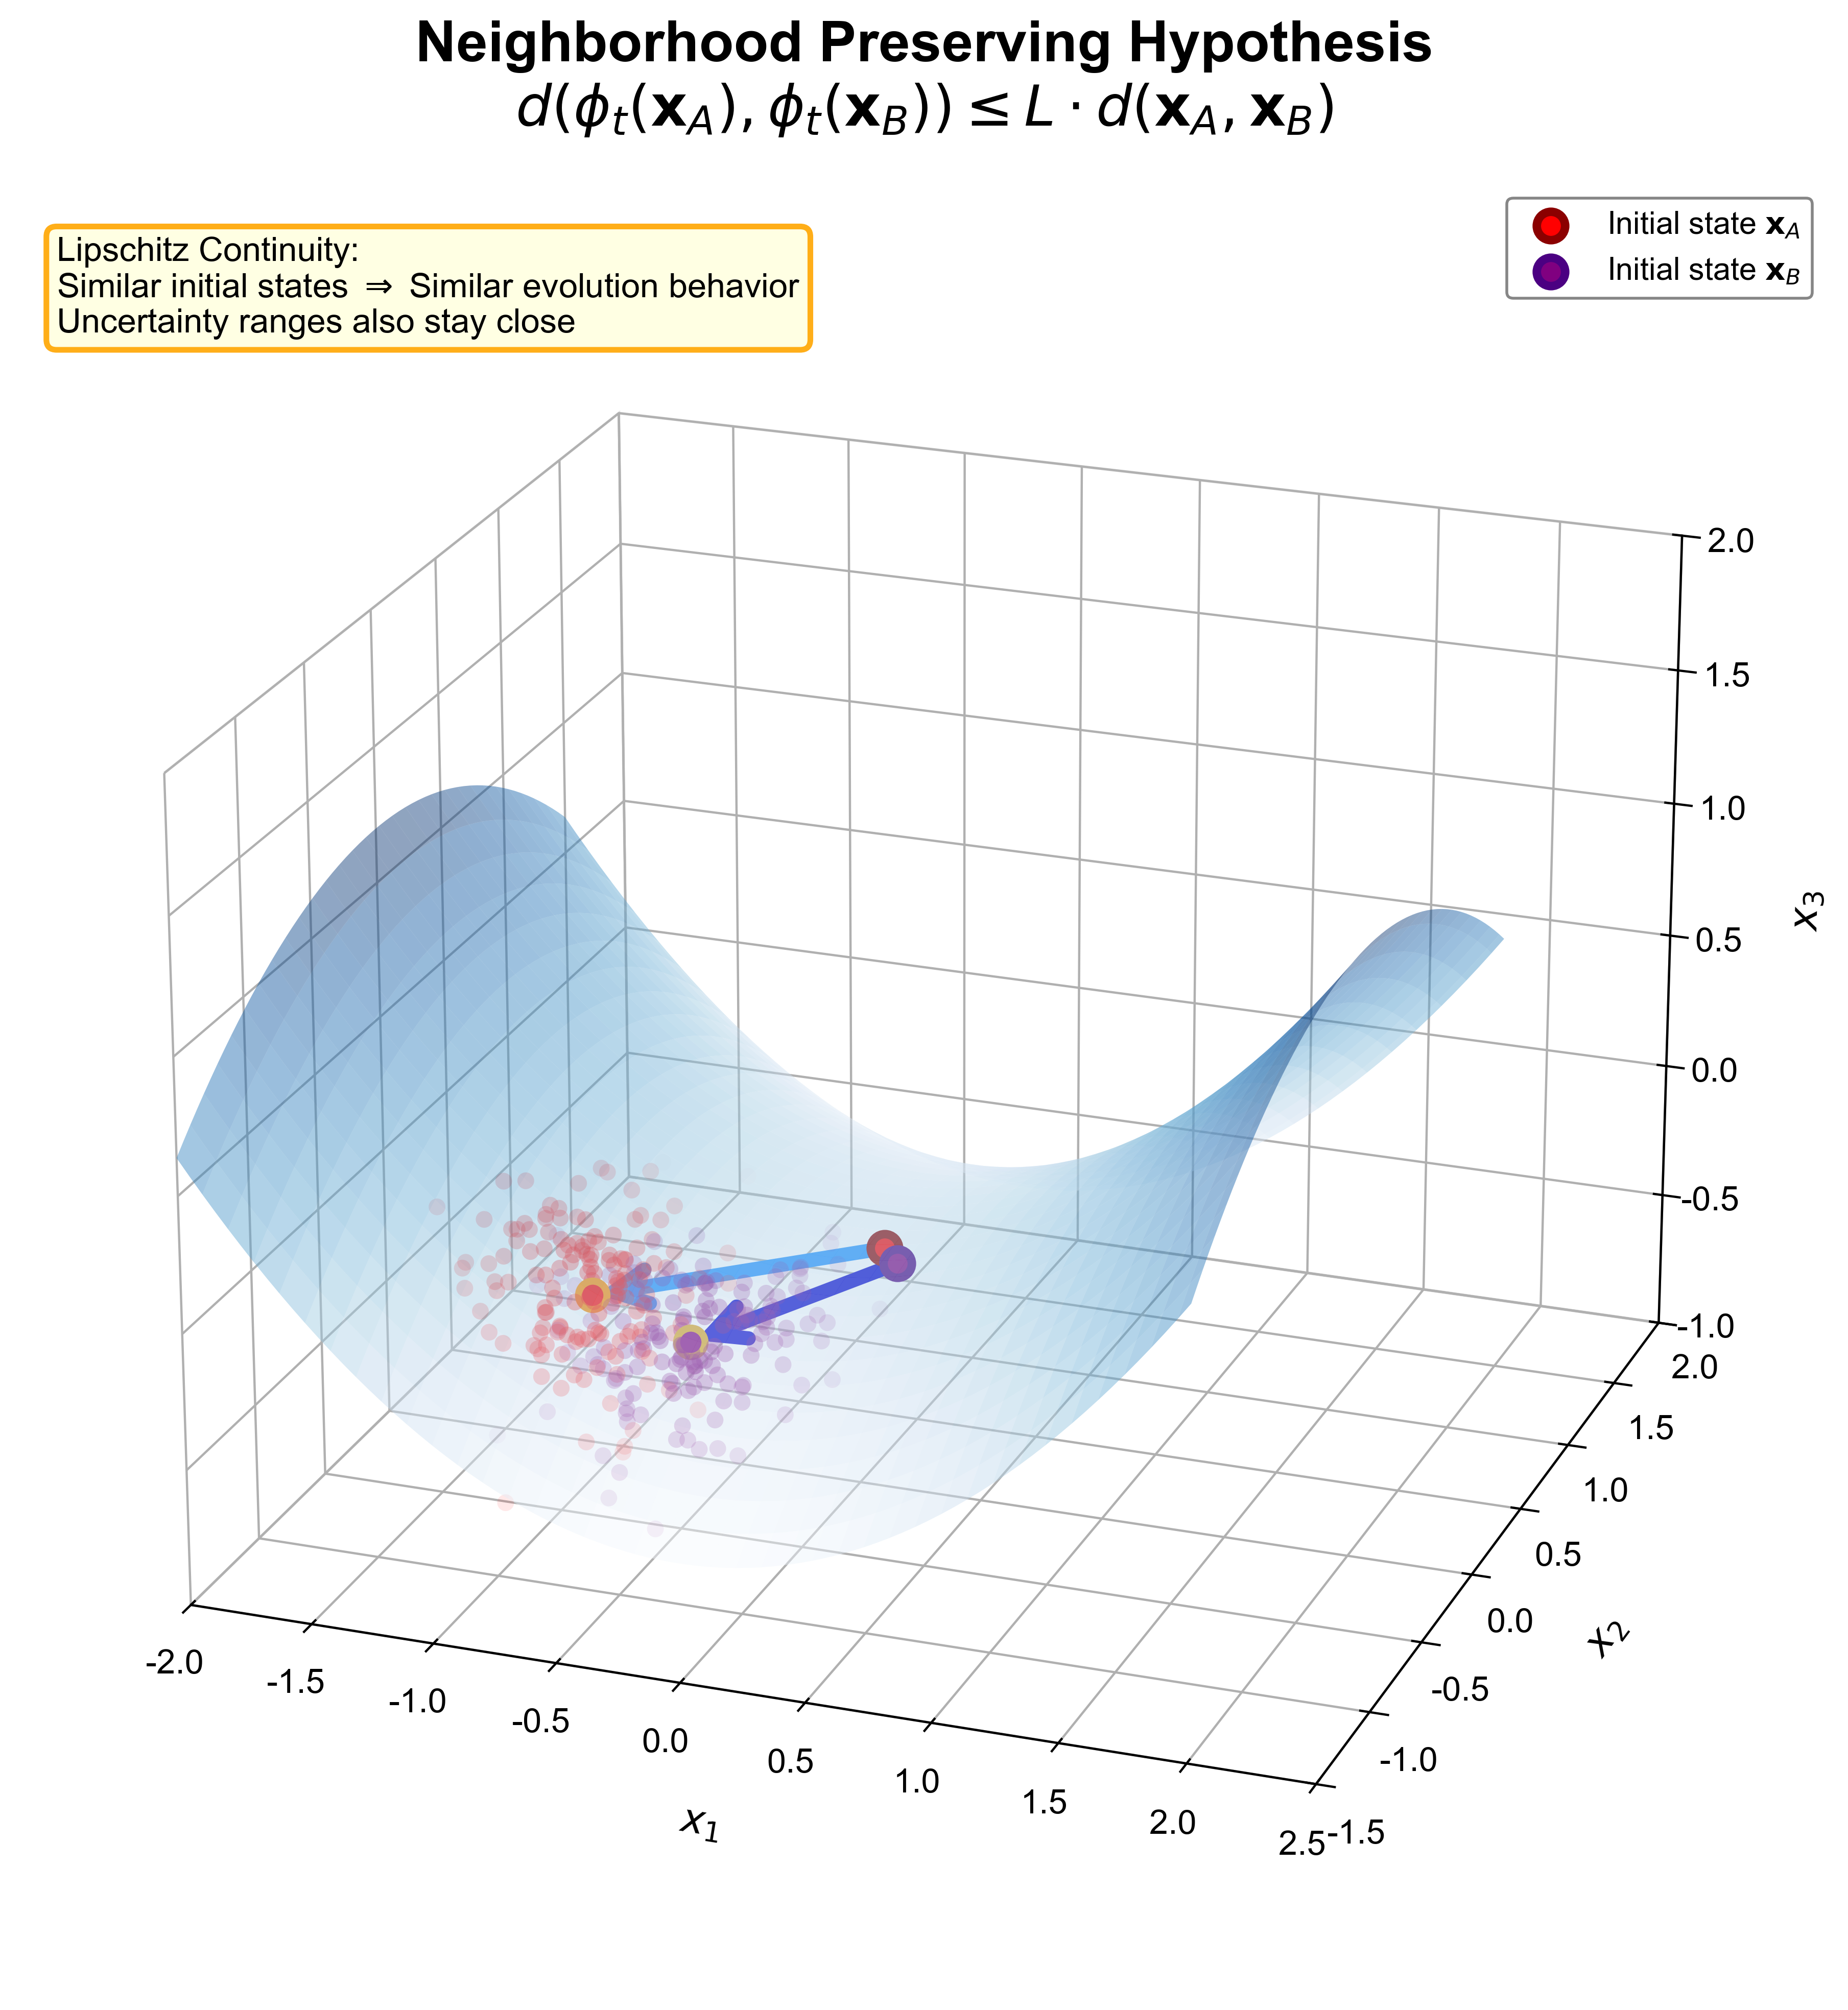
\includegraphics[width=1.00\textwidth]{./assets/neighborhood_preserving.png}
    \caption{近邻假设的几何图景。红色和紫色点代表两初始状态 $\fastvar_A, \fastvar_B$，蓝色和紫色箭头为各自的漂移方向，红色和紫色云团为各自的扩散范围。近邻假设要求: 若初始状态接近，则未来状态的概率分布也应相似。}
    \label{fig:neighborhood_preserving}
\end{figure}

在尝试拟合演化算子 $\evolop_t$ 时，Lipschitz平滑性 \eqref{eq:neighborhood_preserving} 将带来以下好处:
\begin{itemize}
    \item 稳定性 (Stability): 模型具有更高的可预报性极限；
    \item 泛化性 (Generalization): 模型在训练样本的“近邻”内泛化误差可控，预测可靠性高；
    \item 正则化 (Regularization): 较小的Lipschitz常数隐含正则化条件，可以防止模型过拟合；
    \item 鲁棒性 (Robustness): 模型能够容忍一定的观测误差和数值误差。
\end{itemize}

因此，如何构造符合近邻假设，具有较好Lipschitz平滑性的度量 $\metric$，是一个十分重要的问题。
欧氏距离 $\dyndist_{\text{Euclid}}(\fastvar_A, \fastvar_B) = \|\fastvar_A - \fastvar_B\|_2$ 显然不是一个好的选择——物理上相似的状态在欧氏距离下可能很远，物理上差异巨大的状态反而接近。
这里举一个具体例子，我们考虑两个扰动:
\begin{itemize}
    \item 扰动A: ENSO核心区 (约占全球面积的 1\%) 的0.5K海温异常。
    \item 扰动B: 全球每个格点均匀的0.01K温度扰动。
\end{itemize}

按照欧式距离，扰动B的影响更大，即扰动前后状态的距离更远，相似性更低。
但从气候动力学角度理解: 扰动A会在数周内通过Walker环流以遥相关的方式影响全球天气，而扰动B几乎不会产生任何影响。
这说明欧氏距离给出了错误的相似性判断。
如果我们基于此进行建模，模型会认为扰动B的效果“更显著”，这与物理实际完全相反。

\subsection{动力学距离}

Itô SDE \eqref{eq:sde} 描述的动力学系统是随机的。
从初始状态 $\fastvar_0$ 出发，系统在未来 $\predtime$ 时刻的状态 $\fastvar_{\predtime}$ 服从概率分布 $\probdens_{\predtime}(\cdot | \fastvar_0)$。
根据近邻保持假设，\textbf{动力学相似性应由未来状态分布的差异来衡量}。

\begin{definition}[动力学距离]
\label{def:tau_distance}
    固定预报时间 $\predtime > 0$，两初值 $\fastvar_A, \fastvar_B$ 的动力学距离定义为:
    \begin{equation}
    \label{eq:tau_distance}
        d_{\predtime}(\fastvar_A, \fastvar_B) = \sqrt{\predtime} \cdot d_p(\probdens_{\predtime}(\cdot | \fastvar_A), \probdens_{\predtime}(\cdot | \fastvar_B))
    \end{equation}

    其中 $d_p$ 是量化概率分布差异的距离函数，如 Wasserstein 距离 \cite{villani2009optimal}。
    时间权重因子 $\sqrt{\predtime}$ 反映了预报时间对距离度量的自然贡献。
\end{definition}

为推导 $d_{\predtime}$ 的显式形式，需要分析\textbf{SDE的有限时间演化}。
考虑相邻初值 $\fastvar_A, \fastvar_B$，记 $\delta\fastvar_0 = \fastvar_B - \fastvar_A$ 为初始扰动。
我们需要一系列简化假设来使问题在数学上可处理。

\begin{assumption}[局部平稳扩散]
\label{ass:local_stationary_diffusion}
    扩散算子 $\diffop(\fastvar)$ 在小邻域内近似常数:
    \begin{equation}
    \label{eq:local_stationary_diffusion}
        \diffop(\fastvar+\delta\fastvar) \approx \diffop(\fastvar)
    \end{equation}
\end{assumption}

\begin{assumption}[局部线性化]
\label{ass:local_linearization}
    在初值的小邻域 $\|\delta\fastvar_0\|$ 内，漂移项可线性化:
    \begin{equation}
    \label{eq:local_linearization}
        \drift(\fastvar + \delta\fastvar) \approx \drift(\fastvar) + \jacobian_{\drift}(\fastvar) \delta\fastvar
    \end{equation}

    其中 $\jacobian_{\drift} = \frac{\partial \drift}{\partial \fastvar}$ 是雅可比矩阵。
\end{assumption}

\begin{assumption}[适度时间尺度]
\label{ass:moderate_time_scale}
    预报时间 $\predtime$ 满足:
    \begin{equation}
    \label{eq:moderate_time_scale}
        \predtime \ll \frac{1}{\|\jacobian_{\drift}\|} \cdot \frac{L_{\drift}}{\|\delta\fastvar_0\|}
    \end{equation}

    其中 $L_{\drift}$ 是系统特征尺度。这保证线性近似在 $[0, \predtime]$ 内有效。
\end{assumption}

\begin{assumption}[缓变场假设]
\label{ass:slowly_varying_fields}
    雅可比矩阵 $\jacobian_{\drift}(\fastvar_t)$ 和扩散算子 $\diffop(\fastvar_t)$ 在时间尺度 $\predtime$ 内近似常数:
    \begin{equation}
    \label{eq:slowly_varying_fields}
        \jacobian_{\drift}(\fastvar_t) \approx \jacobian_{\drift}(\fastvar_0), \quad \diffop(\fastvar_t) \approx \diffop(\fastvar_0), \quad \forall t \in [0, \predtime]
    \end{equation}
\end{assumption}

以上简化假设的核心思想是进行\textbf{局部时空小扰动近似}: 在空间上，我们假设在一个小邻域内，随机动力学过程的漂移项是线性的，扩散项是恒定的；在时间上，我们要求预报时间 $\predtime$ 相对较短，以至于线性近似依然有效，且动力学过程本身在此期间可视为“冻结”不变。
这些假设在特定条件下是合理的，例如在分析稳定背景场 (如长期气候平均态) 附近的、演化时间较短的小扰动时。

根据假设 \ref{ass:local_stationary_diffusion} 和 \ref{ass:local_linearization}，扰动的演化满足线性化SDE:
\begin{equation}
\label{eq:linearized_sde}
    d(\delta\fastvar_t) = \jacobian_{\drift}(\fastvar_t) \delta\fastvar_t\,dt + \diffop(\fastvar_t) d\wiener_t
\end{equation}

考虑从初值 $\fastvar_A$ 和 $\fastvar_B = \fastvar_A + \delta\fastvar_0$ 出发的两条轨迹。
在假设 \ref{ass:slowly_varying_fields} 下，线性化SDE \eqref{eq:linearized_sde} 是常系数的，其解为:
\begin{equation}
\label{eq:perturbation_solution}
    \delta\fastvar_t = \fundsol_t \delta\fastvar_0 + \int_0^t \fundsol_{t-s} \diffop d\wiener_s
\end{equation}

其中 $\fundsol_t = e^{\jacobian_{\drift}(\fastvar_0) t}$ 是基本解矩阵。
\eqref{eq:perturbation_solution} 表明扰动由动力学指数放大 ($\fundsol_t \delta\fastvar_0$) 和随机扰动累计 ($\int_0^t \fundsol_{t-s}\diffop d\wiener_s$) 两部分构成。

由 \eqref{eq:perturbation_solution} 决定的未来状态概率分布是高斯分布。
具体地，从 $\fastvar_A$ 出发的轨迹在时刻 $\predtime$ 的分布为:
\begin{equation}
\label{eq:gaussian_distribution_of_perturbation_A}
    \probdens_{\predtime}(\cdot|\fastvar_A) = \normdist(\bm{m}_A, \covmat_{\predtime})
\end{equation}

其中 $\bm{m}_A = \fastvar_A + \mathbb{E}\left[\int_0^{\predtime} \drift(\fastvar_A(s)) ds\right]$。
其中协方差为随机扰动的累积效应，根据Itô等距性质 $\mathbb{E}[d\wiener_s d\wiener_s^\top] = I ds$，有:
\begin{equation}
\label{eq:covariance_of_perturbation}
    \covmat_{\predtime} = \mathbb{E}\left[\left(\int_0^{\predtime} \fundsol_{\predtime-s}\diffop d\wiener_s\right) \left(\int_0^{\predtime} \fundsol_{\predtime-s}\diffop d\wiener_s\right)^\top\right] = \int_0^{\predtime} \fundsol_s \difftensor \fundsol_s^\top ds
\end{equation}

类似地，从 $\fastvar_B$ 出发的轨迹在时刻 $\predtime$ 的分布为:
\begin{equation}
\label{eq:gaussian_distribution_of_perturbation_B}
    \probdens_{\predtime}(\cdot|\fastvar_B) = \normdist(\bm{m}_B, \covmat_{\predtime})
\end{equation}

有 $\bm{m}_B = \fastvar_B + \mathbb{E}\left[\int_0^{\predtime} \drift(\fastvar_B(s)) ds\right]$。
注意到 $\probdens_{\predtime}(\cdot|\fastvar_A)$ 和 $\probdens_{\predtime}(\cdot|\fastvar_B)$ 的协方差相同，因为二者的随机扰动都来自标准Wiener过程。

我们取 $d_p(\probdens_{\predtime}(\cdot|\fastvar_A), \probdens_{\predtime}(\cdot|\fastvar_B)) = (\bm{m}_A - \bm{m}_B)^\top \covmat_{\predtime}^{-1} (\bm{m}_A - \bm{m}_B)$，用来描述两个概率分布的差异。
对于共享协方差矩阵的高斯分布，这等价于使用Mahalanobis距离或KL散度 (此时KL散度也是对称的)。

现在计算均值差。
在假设 \ref{ass:local_linearization}下，漂移项满足 $\drift(\fastvar_B(s)) - \drift(\fastvar_A(s)) \approx \jacobian_{\drift} \delta\fastvar_s$，因此:
\begin{align*}
    \bm{m}_B - \bm{m}_A &\approx \delta\fastvar_0 + \mathbb{E}\left[\int_0^{\predtime} \jacobian_{\drift} \delta\fastvar_s ds\right] \\
    &= \delta\fastvar_0 + \mathbb{E}\left[\int_0^{\predtime} \jacobian_{\drift} (\fundsol_s \delta\fastvar_0 + \int_0^s \fundsol_{s-s^\prime} \diffop d\wiener_{s^\prime}) ds\right] \\
    &= \delta\fastvar_0 + \int_0^{\predtime} \jacobian_{\drift} \fundsol_s \delta\fastvar_0 ds + \mathbb{E}\left[\int_0^{\predtime} \int_0^s \jacobian_{\drift} \fundsol_{s-s^\prime} \diffop d\wiener_{s^\prime} ds\right] \\
    &= \delta\fastvar_0 + (\fundsol_{\predtime} - \fundsol_0) \delta\fastvar_0 \\
    &= \fundsol_{\predtime} \delta\fastvar_0
\end{align*}

将均值差代入 \eqref{eq:tau_distance}:
\begin{equation}
\label{eq:tau_distance_final}
    \dyndist_{\predtime}^2(\fastvar_A, \fastvar_B) = \predtime \cdot \delta\fastvar_0^\top \fundsol_{\predtime}^\top \left(\int_0^{\predtime} \fundsol_s \difftensor \fundsol_s^\top ds\right)^{-1} \fundsol_{\predtime} \delta\fastvar_0
\end{equation}

根据定义 \eqref{eq:metric_tensor_def}，导出度量张量:
\begin{equation}
\label{eq:metric_tensor_final}
    \metric_{\predtime}(\fastvar) = \predtime \cdot \fundsol_{\predtime}^\top \left(\int_0^{\predtime} \fundsol_s \difftensor \fundsol_s^\top ds\right)^{-1} \fundsol_{\predtime}
\end{equation}

\subsection{渐近分析}

为理解预报时间 $\predtime$ 对系统几何结构的影响，我们分析度量张量在不同时间尺度下的渐近行为。
我们需要引入对称性与对角化假设，以进一步化简 \eqref{eq:metric_tensor_final}。

\begin{assumption}[对称性与对角化]
\label{ass:commuting_matrices}
    雅可比矩阵 $\jacobian_{\drift}$ 是对称矩阵 ($\jacobian_{\drift} = \jacobian_{\drift}^\top$)，且与扩散张量 $\difftensor$ 可交换 ($[\jacobian_{\drift}, \difftensor] = 0$)。在此条件下，存在正交矩阵 $\eigenvecmat$ 使得:
    \begin{equation}
    \label{eq:simultaneous_diagonalization}
        \jacobian_{\drift} = \eigenvecmat\eigenvalmat \eigenvecmat^\top, \quad \difftensor = \eigenvecmat\diffeigenvalmat \eigenvecmat^\top
    \end{equation}

    其中 $\eigenvalmat = \text{diag}(\eigenval_1, \ldots, \eigenval_N)$ 为实特征值矩阵，$\diffeigenvalmat = \text{diag}(\delta_1, \ldots, \delta_N)$ 为正特征值矩阵。
\end{assumption}

对称性假设要求动力学系统局部上可表示为梯度流 $\drift \approx -\nabla \Phi$，其中 $\Phi$ 是势函数。
这对应于无环流、纯耗散的系统。
在地球系统中，仅部分变量的子系统的雅可比矩阵近似对称，如海洋热含量、土壤湿度等；但对于存在环流、相位传播的子系统，如大气急流、Rossby波等，通常具有非对称的雅可比矩阵。
可交换性进一步要求动力学演化的主方向与随机扰动的主方向对齐，这在一定程度上是合理的，但并非总是成立。
因此，假设 \ref{ass:commuting_matrices} 是较强的简化，我们基于此假设的分析仅提供定性的洞察。

在假设 \ref{ass:commuting_matrices} 下，协方差矩阵 $\covmat_{\predtime}$ 具有简洁的对角化形式。
\begin{align*}
    \covmat_{\predtime} = \int_0^{\predtime} \fundsol_s \difftensor \fundsol_s^\top ds &= \int_0^{\predtime} \eigenvecmat e^{\eigenvalmat s} \eigenvecmat^\top \difftensor \eigenvecmat e^{\eigenvalmat^\top s} \eigenvecmat^\top ds \\
    &= \eigenvecmat \left(\int_0^{\predtime} e^{\eigenvalmat s} (\eigenvecmat^\top \difftensor \eigenvecmat) e^{\eigenvalmat^\top s} ds\right) \eigenvecmat^\top \\
    &= \eigenvecmat \left(\int_0^{\predtime} e^{\eigenvalmat s} \diffeigenvalmat e^{\eigenvalmat^\top s} ds\right) \eigenvecmat^\top \\
    &= \eigenvecmat \left(\text{diag}(\frac{\delta_i}{2 \eigenval_i} (e^{2 \eigenval_i \predtime} - 1))\right) \eigenvecmat^\top
\end{align*}

度量张量 $\metric_{\predtime}$ 为:
\begin{align*}
    \metric_{\predtime} = \predtime \cdot \fundsol_{\predtime}^\top \covmat_{\predtime}^{-1} \fundsol_{\predtime} &= \predtime \cdot \eigenvecmat e^{\eigenvalmat^\top \predtime} \eigenvecmat^\top \eigenvecmat \left(\text{diag}(\frac{\delta_i}{2 \eigenval_i} (e^{2 \eigenval_i \predtime} - 1))\right)^{-1} \eigenvecmat^\top \eigenvecmat e^{\eigenvalmat \predtime} \eigenvecmat^\top \\
    &= \predtime \cdot \eigenvecmat e^{\eigenvalmat^\top \predtime} \left(\text{diag}(\frac{2 \eigenval_i}{\delta_i} \frac{1}{e^{2\eigenval_i \predtime} - 1})\right) e^{\eigenvalmat \predtime} \eigenvecmat^\top \\
    &= \eigenvecmat \left(\text{diag}\left(\frac{2 \eigenval_i \predtime}{\delta_i} \frac{e^{2\eigenval_i \predtime}}{e^{2\eigenval_i \predtime} - 1}\right)\right) \eigenvecmat^\top
\end{align*}

度量对角元为:
\begin{equation}
\label{eq:metric_tensor_diagonal_element}
    [\metric_{\predtime}]_{ii} = \frac{2\eigenval_i \predtime}{\delta_i} \frac{e^{2\eigenval_i\predtime}}{e^{2\eigenval_i\predtime} - 1}
\end{equation}

图 \ref{fig:metric_vs_tau} 展示了不同 $\eigenval_i$ 取值下度量对角元随预报时间 $\predtime$ 的演化。
\begin{figure}[htbp]
    \centering
    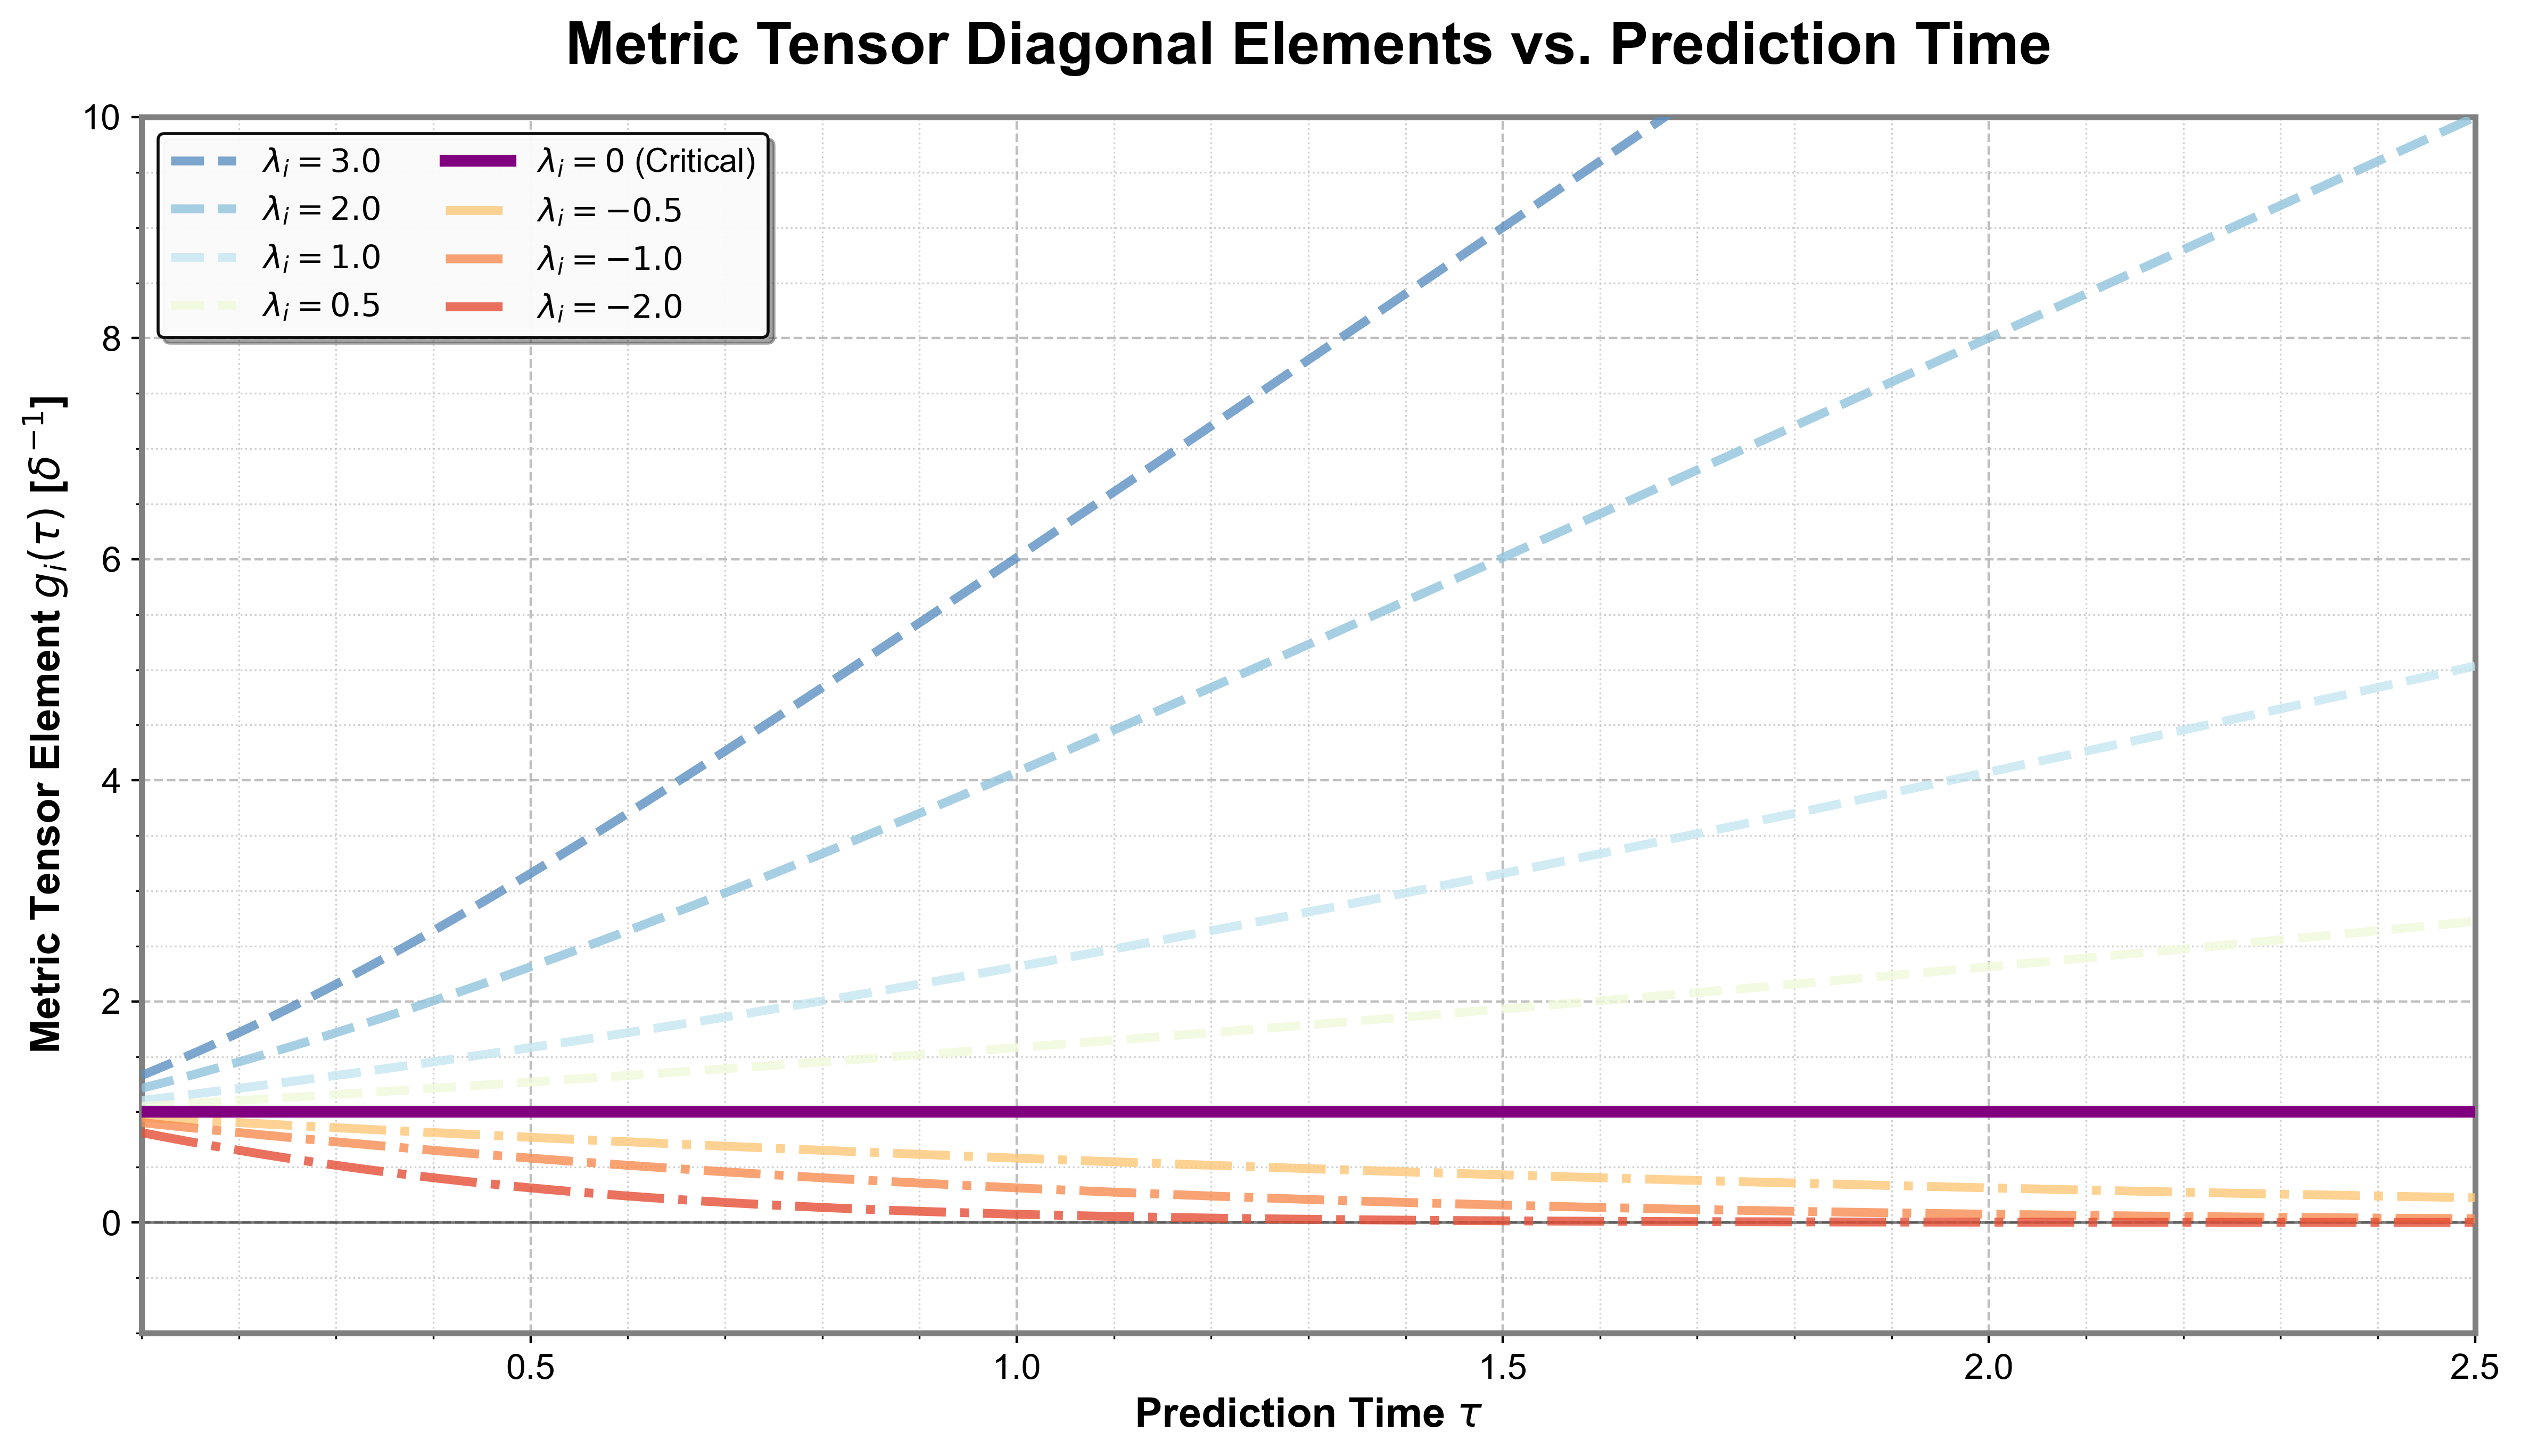
\includegraphics[width=1.00\textwidth]{./assets/metric_tensor_elements.png}
    \caption{度量张量对角元素随预报时间的演化规律。紫色粗线对应中性方向 ($\lambda = 0$)，蓝色系对应稳定方向 ($\lambda < 0$)，红色系对应不稳定方向 ($\lambda > 0$)。}
    \label{fig:metric_vs_tau}
\end{figure}

\textbf{1. 中性方向 ($\eigenval_i = 0$): 准守恒模态}

当 $\eigenval_i = 0$ 时，对应于动力学系统的\textbf{中性方向}，初始扰动既不增长也不衰减。
利用L'Hôpita 法则:
\begin{equation}
\label{eq:metric_neutral}
    [\metric_{\predtime}]_{ii} = \lim_{\eigenval_i \to 0} \frac{2 \eigenval_i \predtime}{\delta_i} \cdot \frac{e^{2 \eigenval_i \predtime}}{e^{2 \eigenval_i \predtime} - 1} = \frac{1}{\delta_i}
\end{equation}

\begin{figure}[htbp]
    \centering
    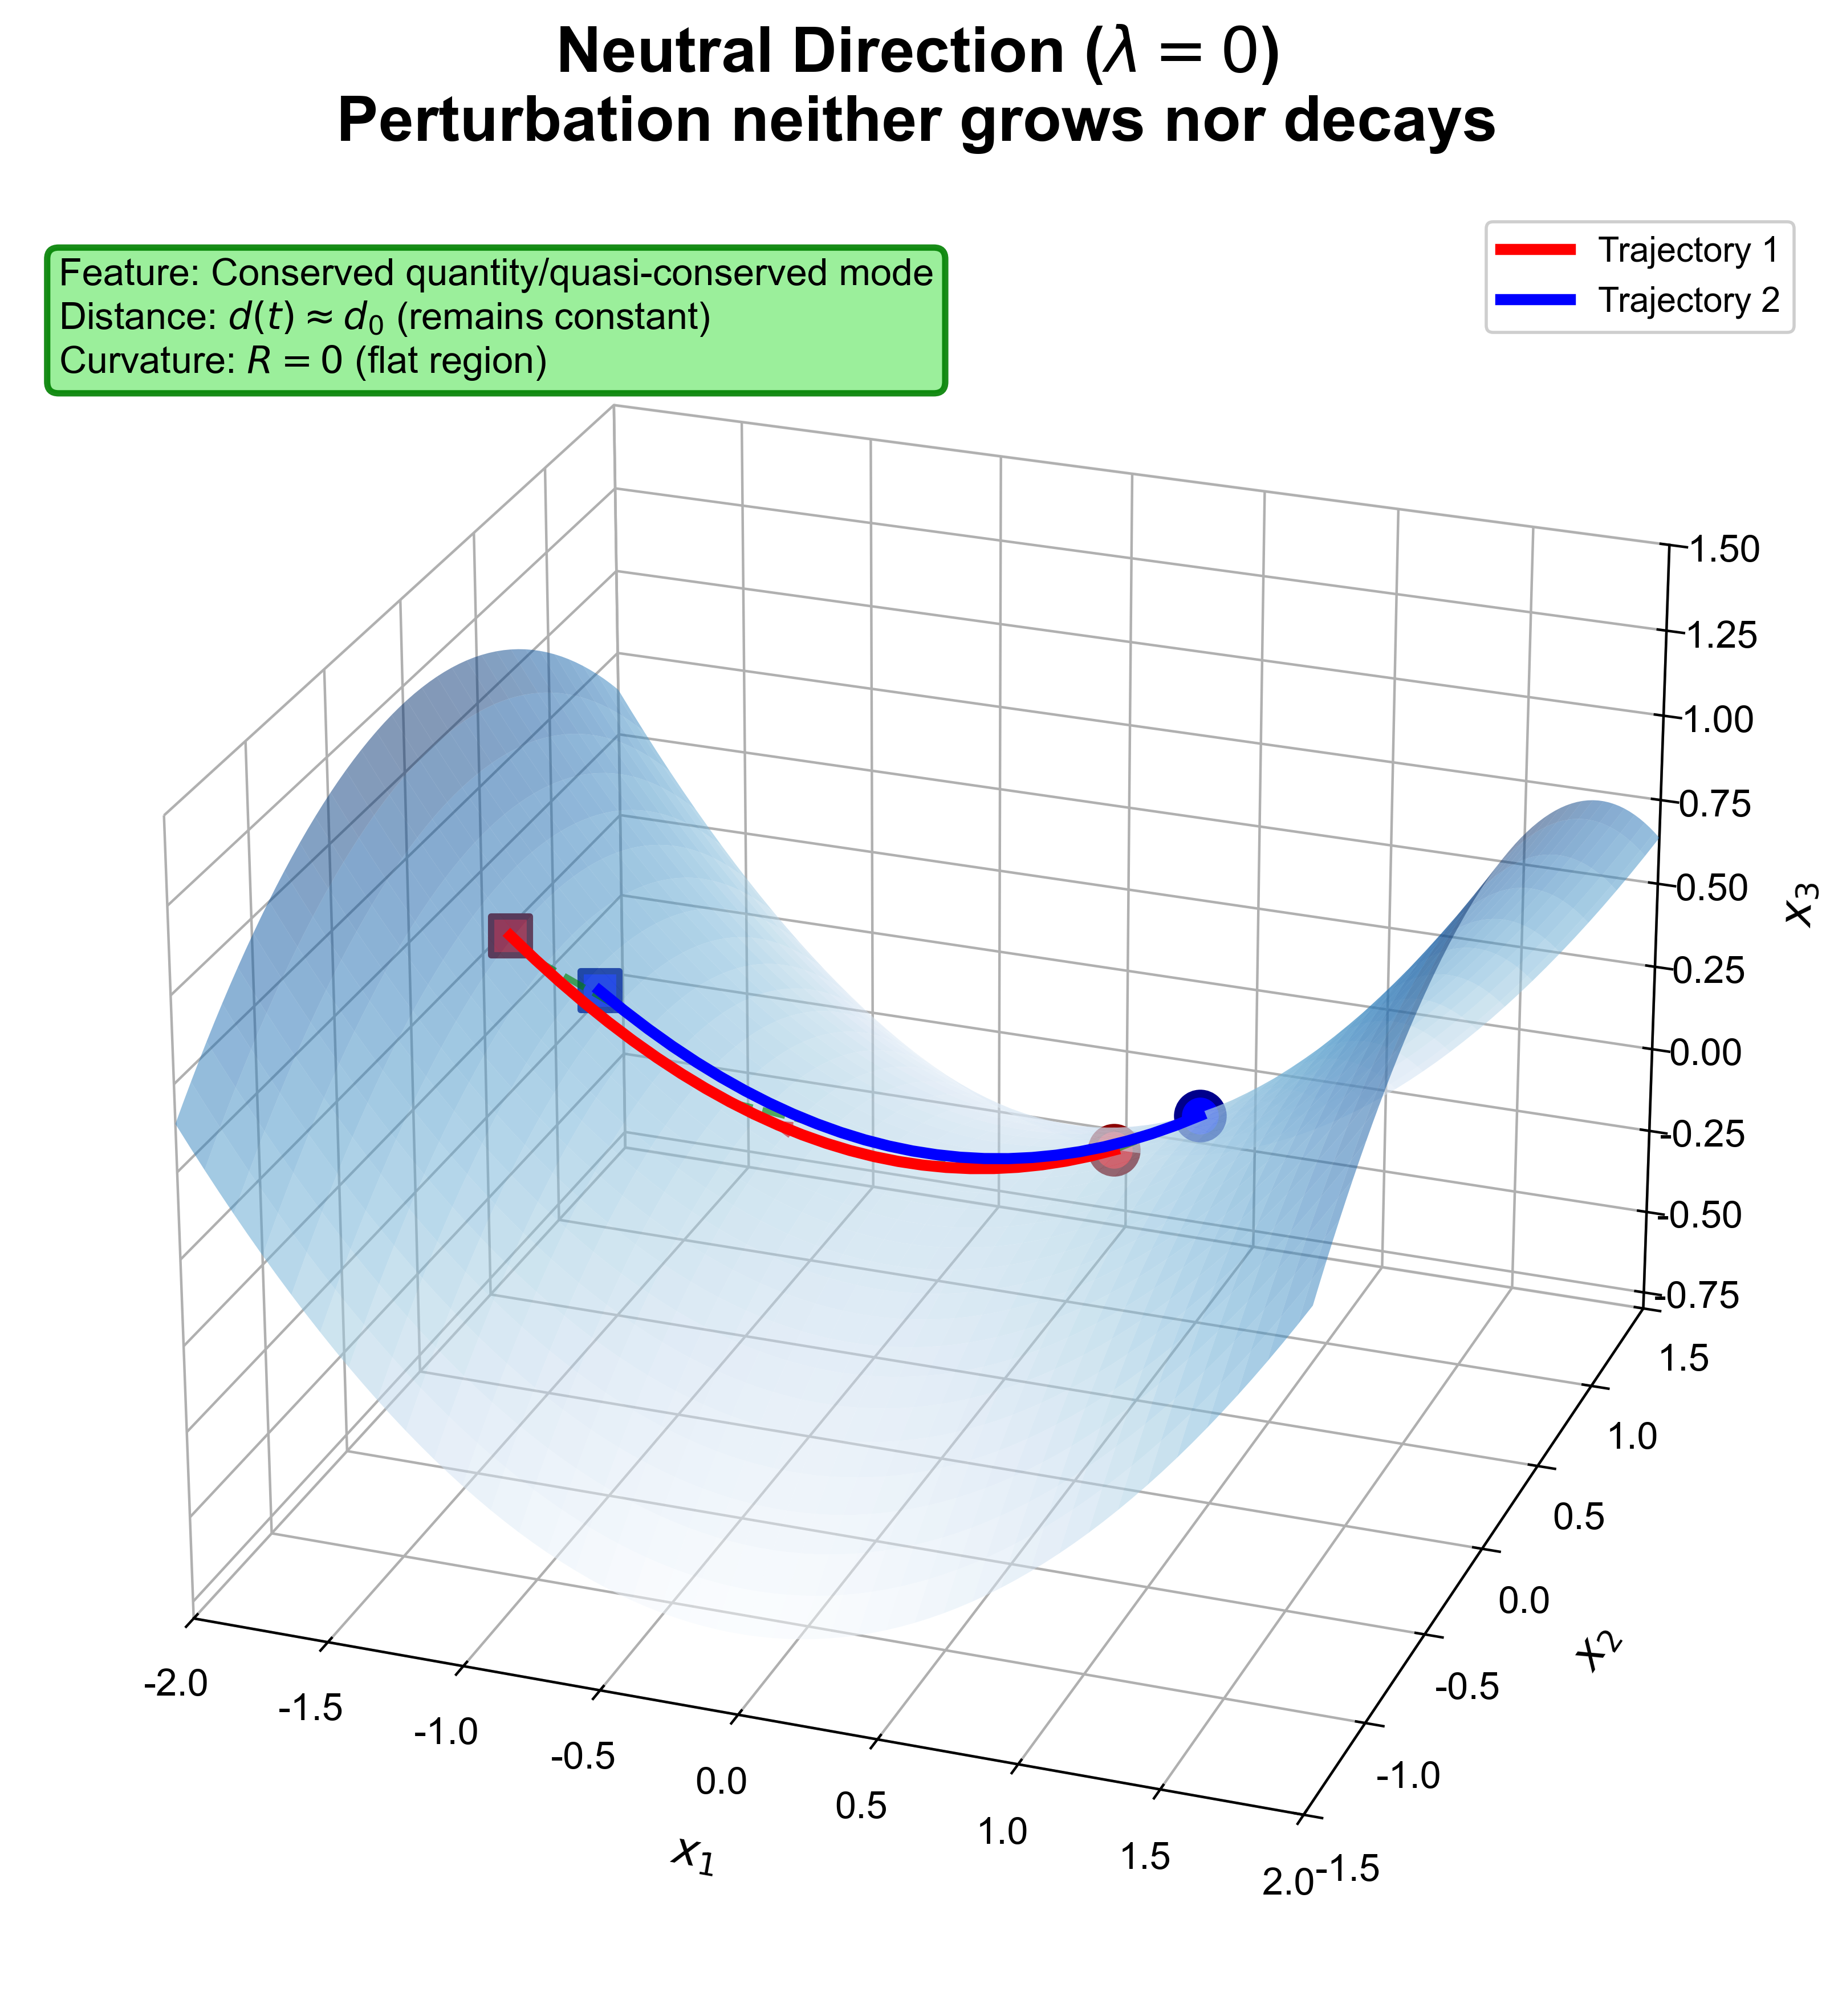
\includegraphics[width=0.56\textwidth]{./assets/neutral_direction.png}
    \caption{中性方向的几何图景。两条轨迹 (红色和蓝色) 从接近的初值出发，沿中性方向演化，距离保持恒定。绿色虚线标示不同时刻的距离。}
    \label{fig:neutral_direction}
\end{figure}

如图 \ref{fig:metric_vs_tau} 和 \ref{fig:neutral_direction} 所示，中性方向的度量保持常数，与预报时间 $\predtime$ 无关。
曲率在该方向上为零，对应流形上的“平坦区域”。
不存在混沌效应的作用，动力学距离完全由扩散控制: $d_{\predtime} \sim \sqrt{1 / \delta_i}$。
时间权重 $\sqrt{\predtime}$ 恰好抵消了扩散导致的 $1/\sqrt{\predtime}$ 衰减。

物理上，中性方向对应\textbf{准守恒模态}，如地转平衡态中的位涡守恒、绝热过程中的熵守恒、海洋盐度-温度补偿关系等。
这些模态的可预报性可以保持较长时间，是季节至年际预报的重要基础 \cite{majda2012climate}。

\textbf{2. 稳定方向 ($\eigenval_i < 0$): 吸引子}

当 $\eigenval_i < 0$ 时，对应于\textbf{稳定方向}。
设 $\eigenval_i = -\mu_i$，其中 $\mu_i > 0$，度量对角元为:
\begin{equation}
\label{eq:metric_stable}
    [\metric_{\predtime}]_{ii} = \frac{2 \mu_i \predtime}{\delta_i} \frac{e^{-2 \mu_i \predtime}}{1 - e^{-2 \mu_i \predtime}} \xrightarrow{\predtime \to \infty} 0
\end{equation}

\begin{figure}[htbp]
    \centering
    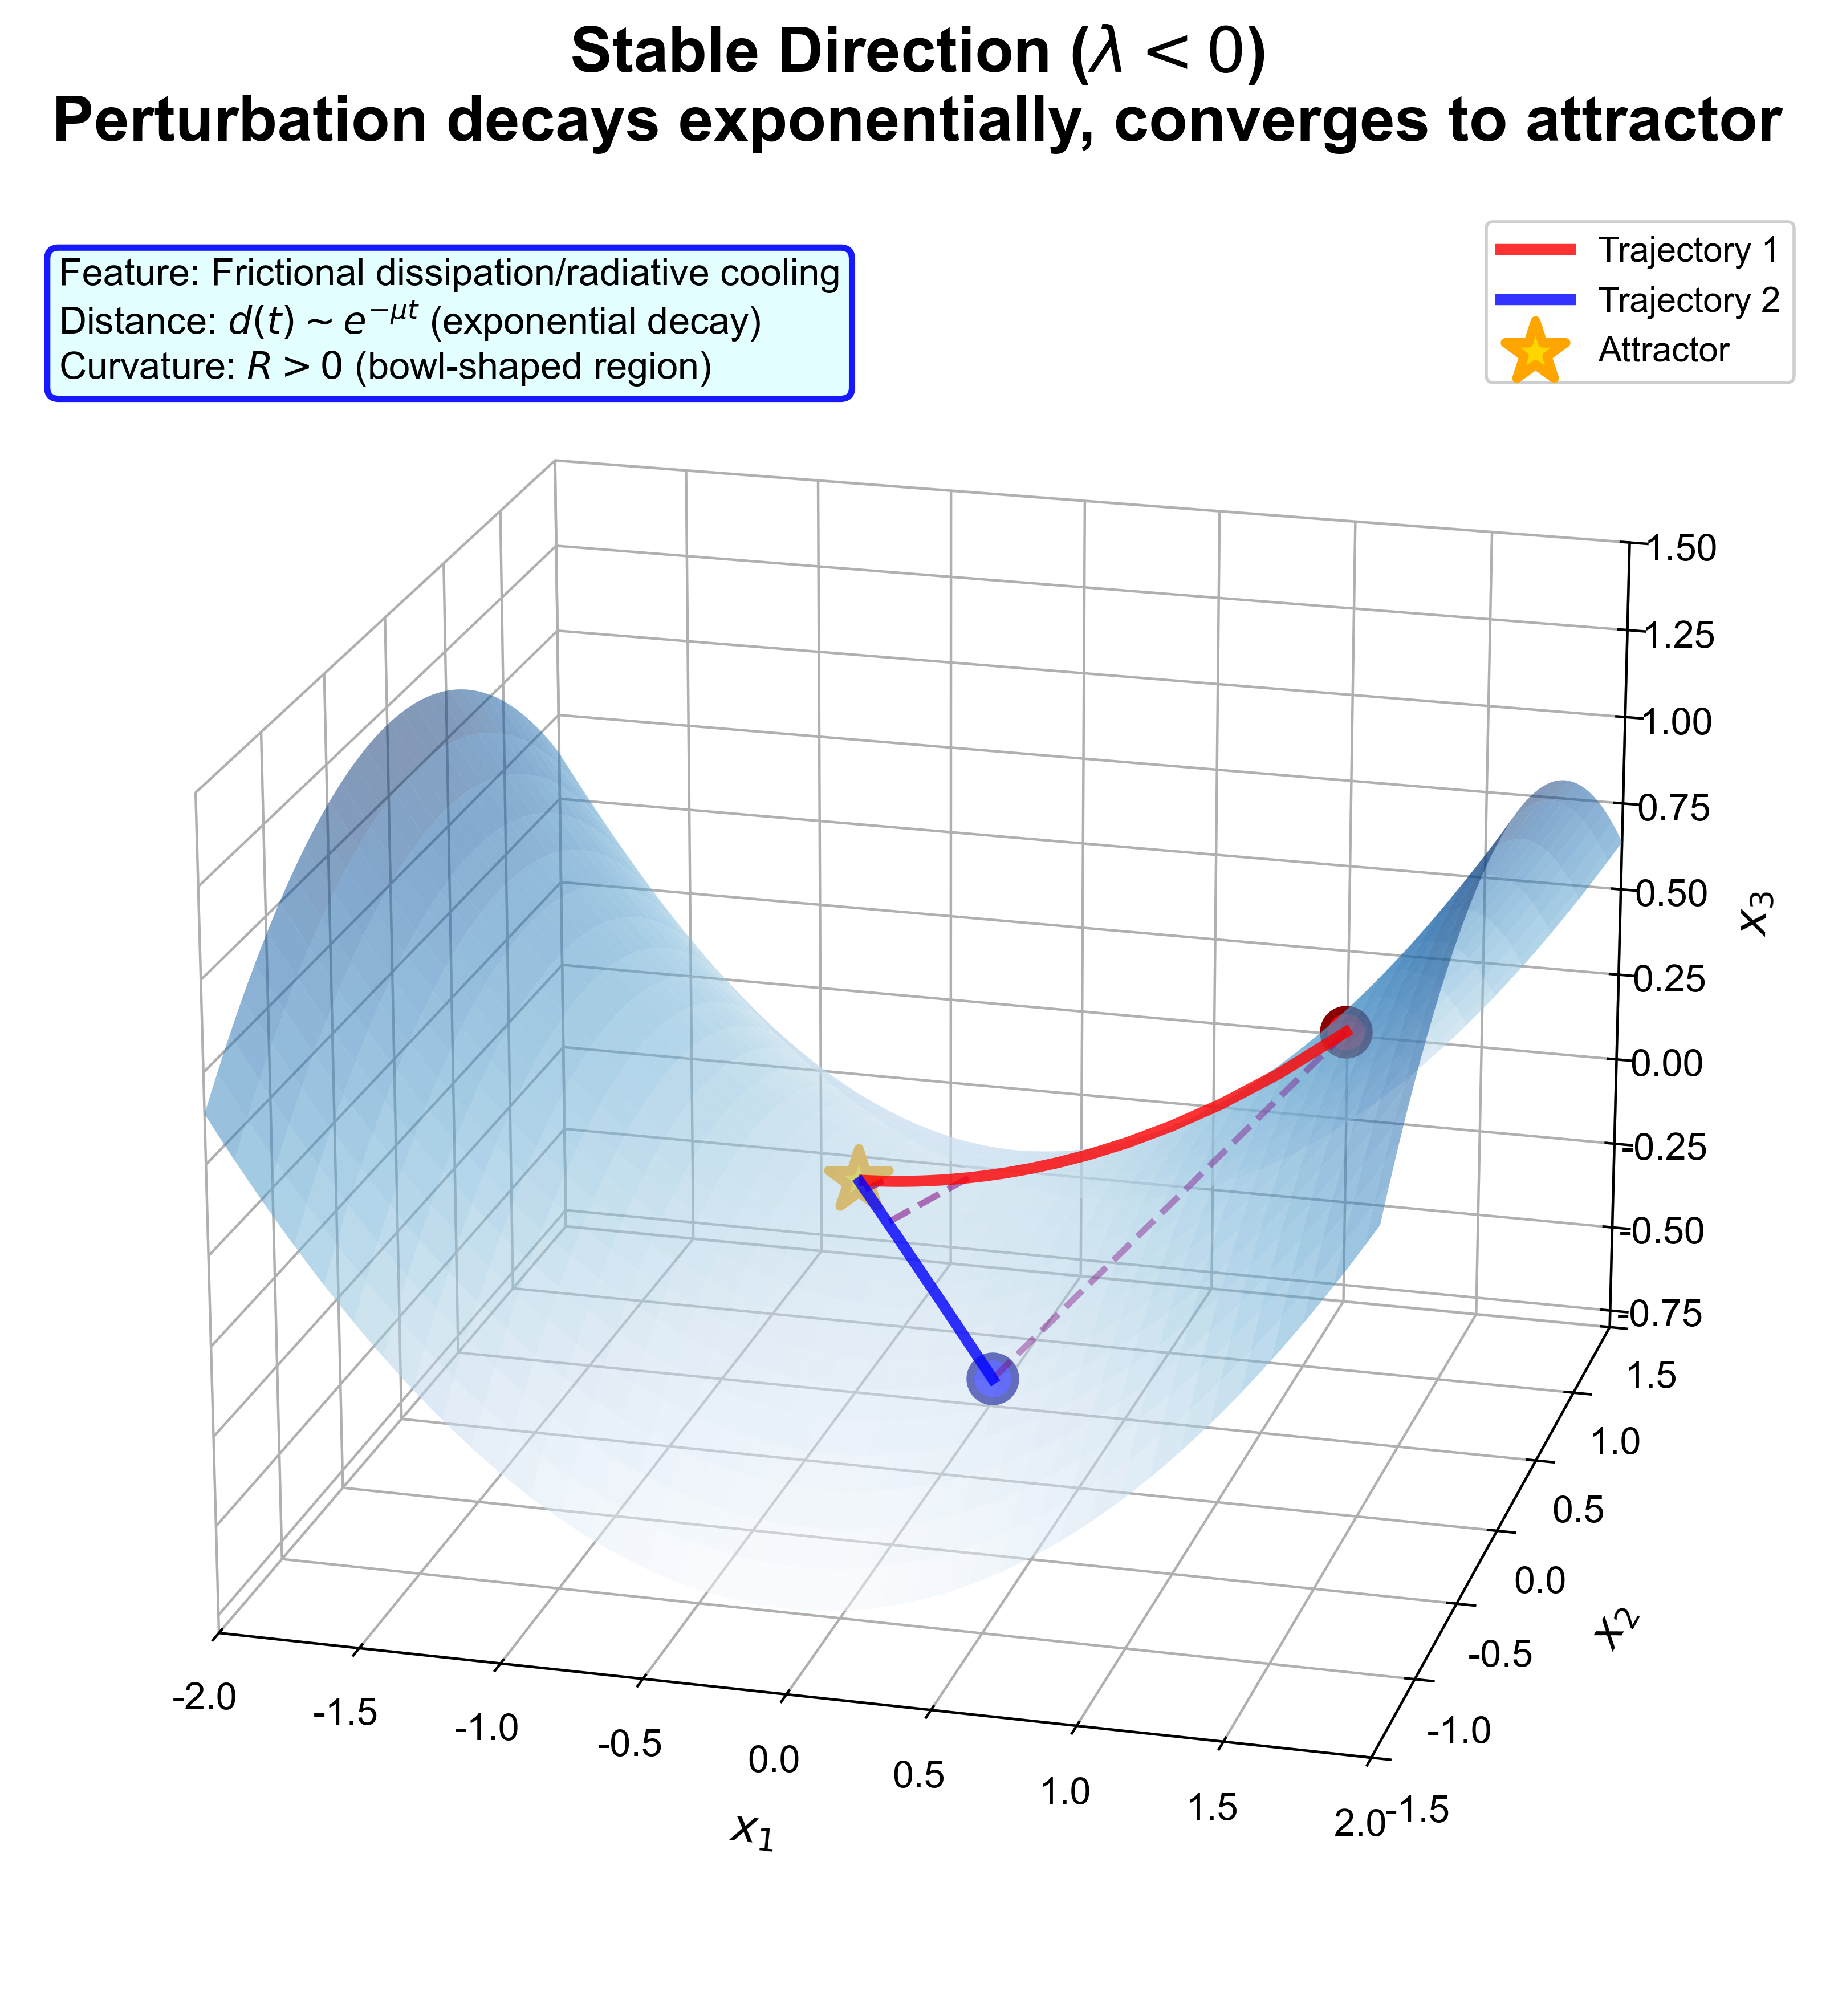
\includegraphics[width=0.56\textwidth]{./assets/stable_direction.png}
    \caption{稳定方向的几何图景。两条轨迹从不同初值出发，沿稳定方向演化，指数收敛到同一吸引子 (金色五角星)。紫色虚线标示距离随时间指数衰减。}
    \label{fig:stable_direction}
\end{figure}

如图 \ref{fig:metric_vs_tau} 和 \ref{fig:stable_direction} 所示，稳定方向的度量呈指数下降，直至趋于零。
曲率为正，对应流形上的“碗状”区域。
沿稳定方向的初始扰动以指数速率 $\mu_i$ 衰减，两条初始接近的轨迹迅速收敛至同一\textbf{吸引子 (Attractor)}。
该方向上的不确定性对未来状态的影响逐渐消失，被吸引子的收缩性抵消。

物理上，稳定方向对应大气中的摩擦耗散、辐射冷却、海洋中的深层混合等过程 \cite{palmer1993extended}。
例如，边界层湍流摩擦导致近地风速扰动快速衰减 ($\meanval \sim 1\,\text{day}^{-1}$)。
吸引子的存在保证了气候系统的\textbf{韧性 (Resilience)}: 即使遭受一定程度的外部冲击，地球系统最终仍将恢复到吸引子上。

\textbf{3. 不稳定方向 ($\eigenval_i > 0$): 混沌效应}

当 $\eigenval_i > 0$ 时，对应于\textbf{不稳定方向}。
雅可比矩阵 $\jacobian_{\drift}$ 的正特征值表征初始扰动的指数增长率 (即Lyapunov指数)，是\textbf{混沌效应 (Chaos Effect)}的动力学根源。

度量对角元为:
\begin{equation}
\label{eq:metric_unstable}
    [\metric_{\predtime}]_{ii} = \frac{2 \eigenval_i \predtime}{\delta_i} \frac{e^{2 \eigenval_i \predtime}}{e^{2 \eigenval_i \predtime} - 1} \xrightarrow{\predtime \to \infty} \frac{2\eigenval_i \predtime}{\delta_i}
\end{equation}

\begin{figure}[htbp]
    \centering
    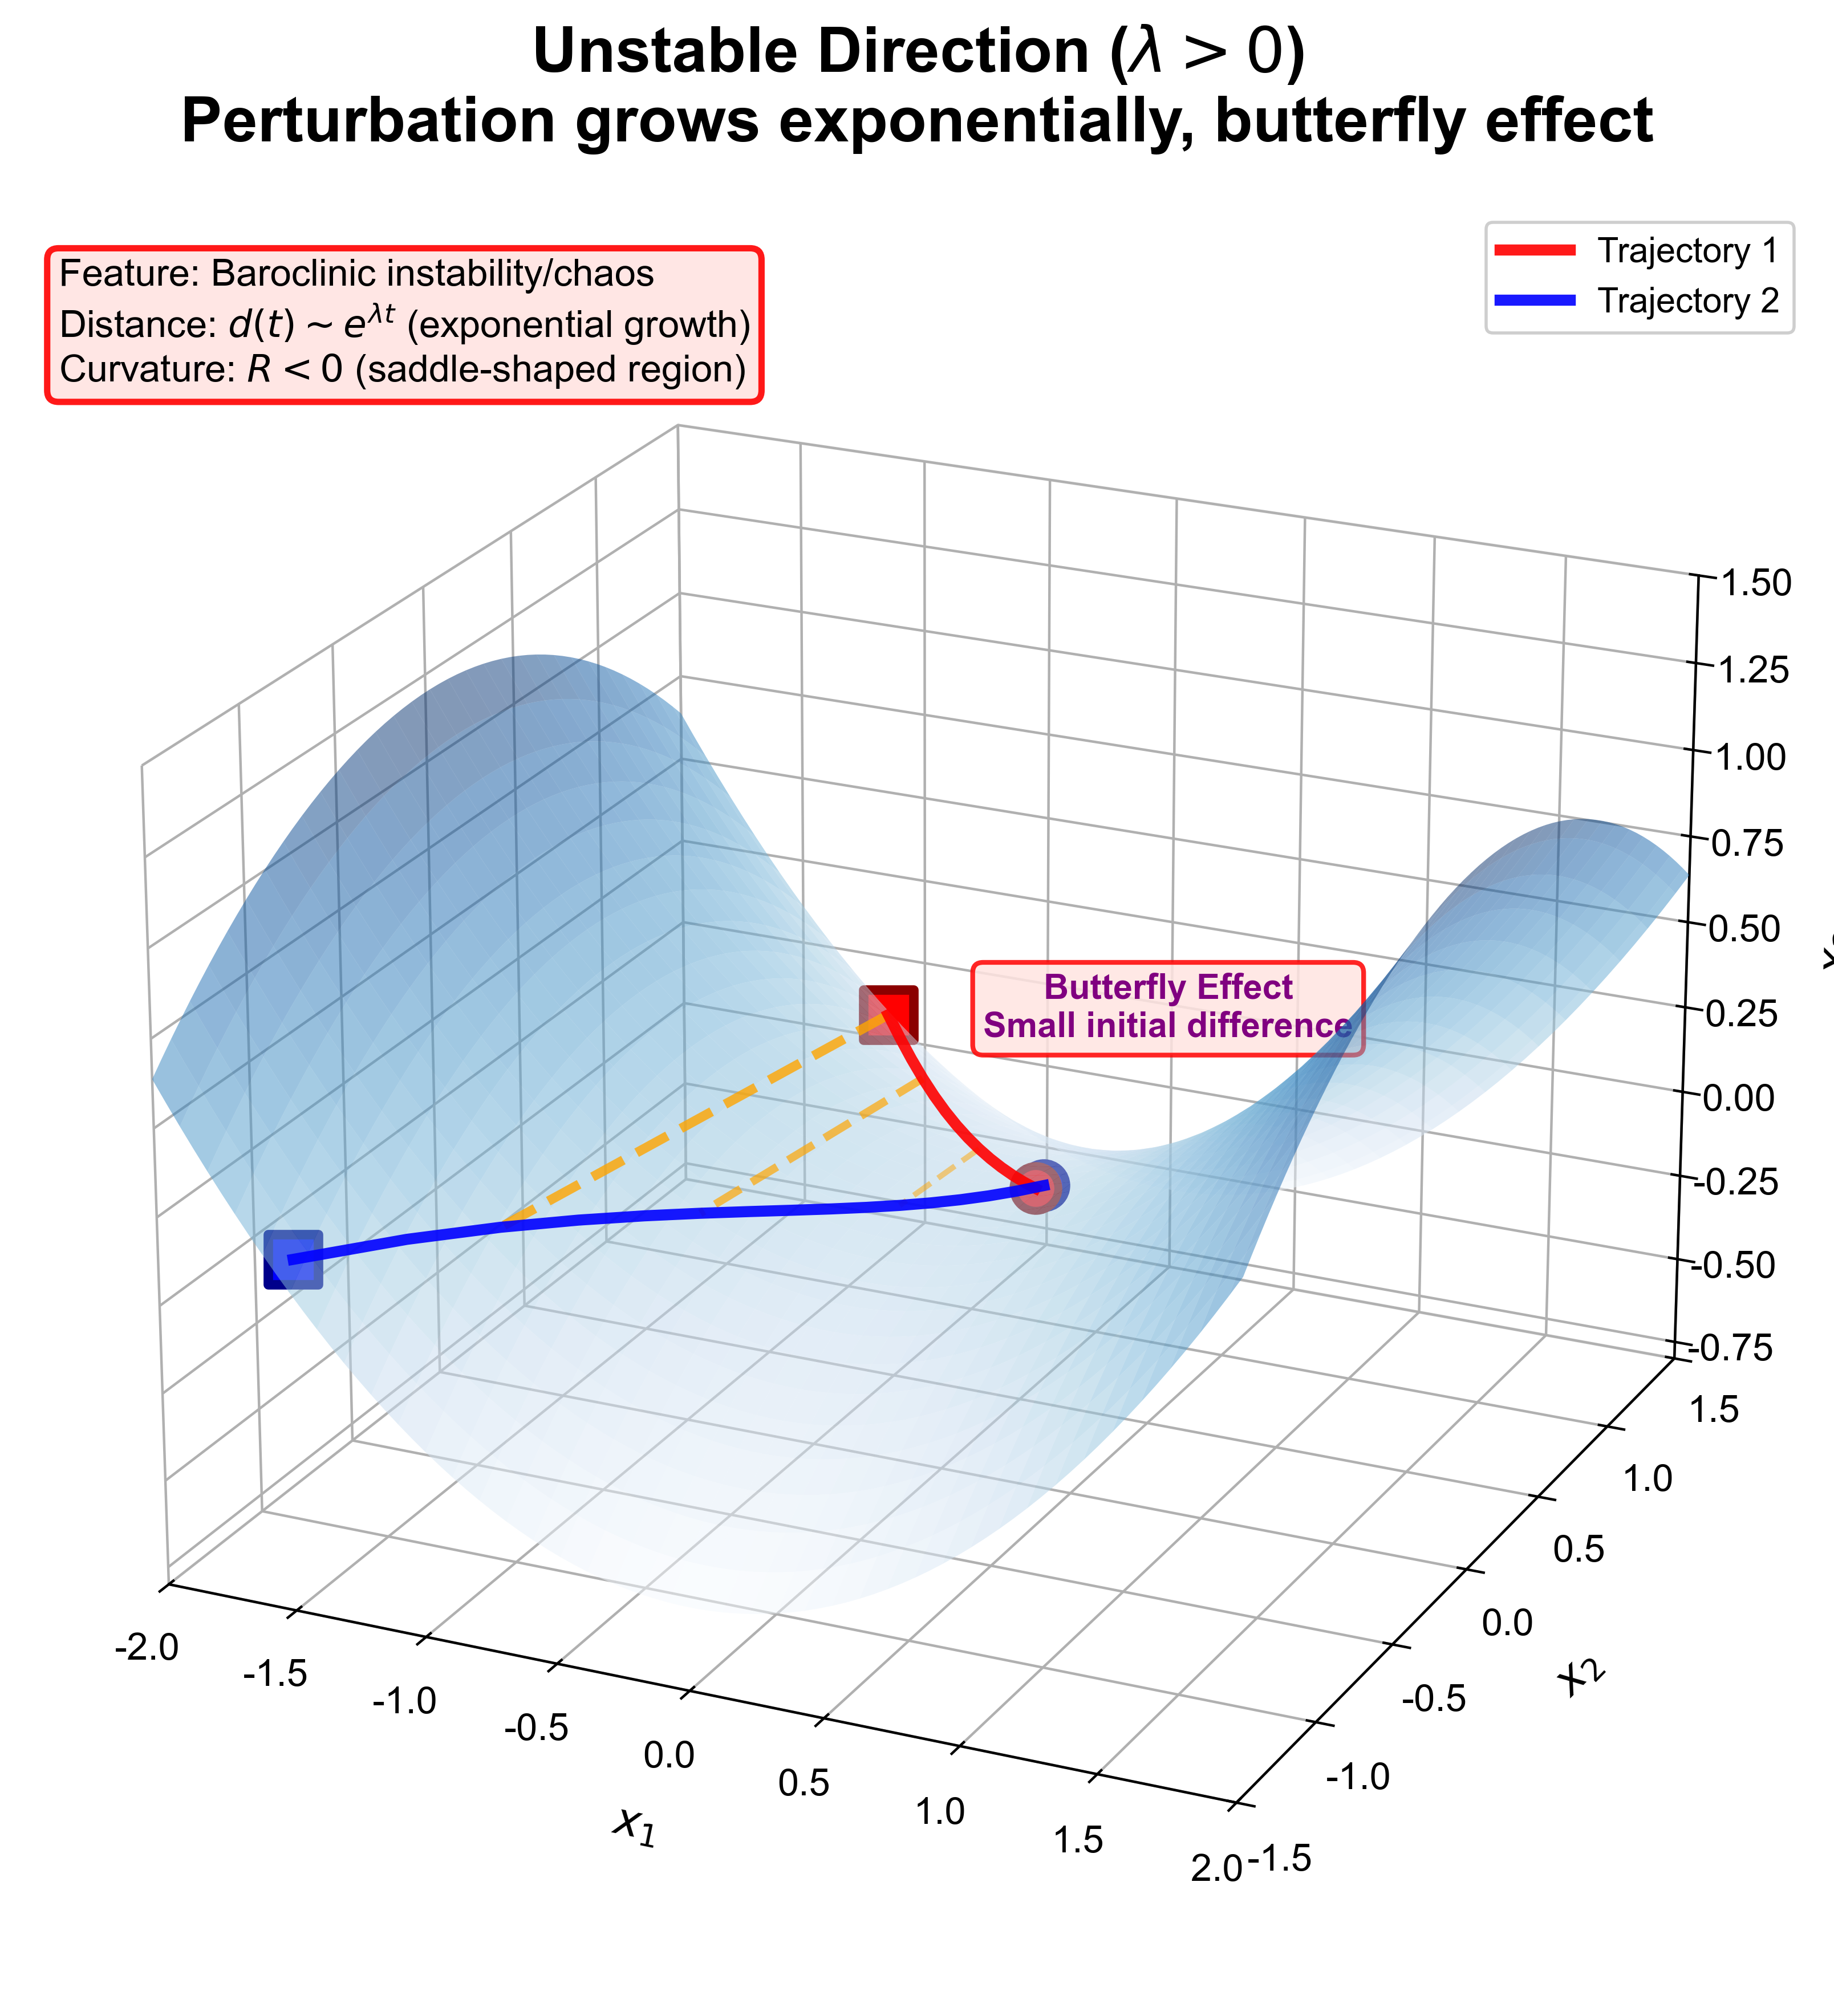
\includegraphics[width=0.56\textwidth]{./assets/unstable_direction.png}
    \caption{不稳定方向的几何图景 (蝴蝶效应)。两条轨迹从极其接近的初值出发 (红色和蓝色点几乎重合)，沿不稳定方向演化，距离指数发散。橙色虚线标示距离随时间指数增长。}
    \label{fig:unstable_direction}
\end{figure}

如图 \ref{fig:metric_vs_tau} 和 \ref{fig:unstable_direction} 所示，不稳定方向的度量呈线性增长趋势。
比例系数 $2\eigenval_i / \delta_i$ 为内禀的可预报性因子，量化了动力学混沌效应与随机噪声扩散的竞争。
曲率在该方向上为负，且绝对值将随着预报时间 $\predtime$ 的增大而线性增大，像是流形上一片正在被不断扭曲的“鞍形区域”。
这是对Lorenz \cite{lorenz1963deterministic} 提出的“蝴蝶效应”的微分几何表述。
系统的可预报性将随着预报时间的拉长而迅速降低，成为预报技巧损失的主导因素。

物理上，不稳定方向对应大气动力学中的正压不稳定和斜压不稳定模态。
初始扰动沿此方向呈指数增长，表现为天气尺度扰动的快速发展 (如锋生、气旋加深) \cite{palmer1993extended}。
